\documentclass[a4paper, 12pt]{article}
\usepackage[francais]{babel}
\usepackage{graphicx}
\usepackage[utf8]{inputenc}
\usepackage[T1]{fontenc}
\usepackage{fancyhdr}
\usepackage[margin=1in]{geometry}
\usepackage{amsmath}
\usepackage{amssymb}
\author{Thibault \bsc{BEZIERS LA FOSSE}}
\date{}
\title{Étude et Comparaison d'Algorithmes}



\pagestyle{fancy}
\begin{document}

\maketitle
\clearpage

\tableofcontents
\clearpage

\section{Introduction}
Ce projet en six séances à pour objectif d'implémenter des algorithmes, afin de calculer leurs complexités et comparer les performances. 
Quatre algorithmes sont à notre disposition, ce compte rendu les traitera dans l'ordre donné. Seront expliqués:
\begin{itemize}
\item[L'implémentation]
\item[La complexité théorique]
\item[Les résultats d'exécutions]
\item[L'analyse des résultats]
\item[Le comparatif des résultats théoriques et expérimentaux]
\end{itemize}
\subsection{Objectif}
Les quatre algorithmes à implémenter consistent à trouver la suite de termes du tableau dont la somme est maximum. 
Les éléments du tableau sont choisis de manière aléatoire, et nous exécuterons nos algorithmes sur des tableaux de tailles variables, en commençant par des tableaux de moins d'une dizaine d'éléments, à des tableaux qui en contiennent des dizaines de milliers.  
\subsection{Outils utilisés}
Le langage de programmation à utiliser pour ce projet étant libre, j'ai choisi de m'orienter vers le C++. D'abord pour une raison pratique, l'université nous fait régulièrement utiliser ce langage. Ensuite pour des raisons de performances, car C++ reste un langage assez efficace pour effectuer des opérations comme celles de ce projet.
Le compilateur utilisé est G++, avec la librairie C++11. Effectivement, G++ est disponible à l'université, et la librairie C++11 offre des méthodes efficaces, et surtout pratiques pour manipuler des tableaux. 
\subsection{Structure du programme}
Quatre algorithmes étant à implémenter, j'ai choisi de créer une arborescence de classes sur un seul niveau. En haut, une classe abstraite implémentant les principales méthodes nécessaires à l’exécution des algorithmes, et en bas les algorithmes qui redéfinissent la méthode de calcul de la méthode \bsc{MaxSomme}:

\begin{figure}[h]
	\centering
	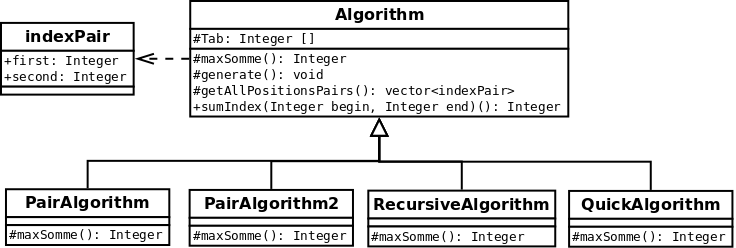
\includegraphics[scale=0.3]{diagramme.png}
	\caption{Diagramme UML du programme}
	\label{uml}	
\end{figure}

 
Les algorithmes implémentés doivent calculer la différence entre deux cases du tableau. J'ai décidé de créer une structure très simple, appelée IndexPair, contenant deux entiers: first et second, contenant chacun une cellule du tableau:
\begin{verbatim}
struct {
    int first;
    int second;
}
\end{verbatim}

\subsection{Méthodes principales}
Voici les méthodes, ainsi que leurs complexités respectives, qui sont implémentées dans la classe mère pour être ensuite réutilisées dans tous les algorithmes.
\subsubsection{Méthode: generate(Int n): void}
Cette méthode remplit le tableau avec des nombres aléatoires entre -1000 et 1000. Le paramètre $n$ correspond au nombre de cases désirées pour le tableau, et l'algorithme est très simple:
\begin{verbatim}
Pour i allant de 1 à n:
    tab[i] = random(-1000, 1000)
FinPour
\end{verbatim}
La complexité de la fonction random étant constante, cette méthode a une complexité en $\theta (n)$.

\subsubsection{Méthode: getAllPositionPairs()}
Cette méthode calcule toutes les paires possibles en fonction de la taille du tableau. Par exemple pour un tableau [1, 2, 3, 4], elle renverra un tableau qui contient les paires {[1,2], [1, 3], [1, 4], [2, 3], [2, 4], [3, 4]}
L'algorithme est le suivant:
\begin{verbatim}
Paires = []                         Coût: 1 
Pour i allant de 1 à n-1:           Coût: Voir ci-dessous
    Pour j allant de i+1 à n:       Coût: Voir ci-dessous
        Paires.ajouter([i, j])      coût: 1
    FinPour
FinPour
\end{verbatim}
Cet algorithme est assez simple à implémenter, et nécessaire pour plusieurs des algorithmes de MaxSomme. 
Détail du calcul de sa complexité théorique:

Boucle 1: effectuée $n-1$ fois

Boucle 2: effectuée $(n-2) + (n-3) + (n-4) + ... + n-(n-1)$ fois
soit $1 + 2 + ... + n-2$

Ainsi on a la somme des entiers de 1 à n-2 qui peut être calculée ainsi:

\begin {center}
$\frac{(n-3)(n-2)}{2}$
\end{center}

Sans détailler le calcul, on voit immédiatement qu'on a un produit de $n$, on peut donc en déduire une complexité en $O(n^2)$.

\subsubsection{Méthode: sumIndex(Int a, Int b): int}
Cette méthode est simple, elle prend deux entiers en paramètre, qui sont chacun un indice du tableau, et calcule la somme des cases du tableau entre ces deux indices. Cet algorithme est récursif:
\begin{verbatim}
Si debut == fin:
    Retourner fin
Sinon 
    Retourner tab[debut] + sumIndex(debut+1, fin)
Fin
\end{verbatim}
On a une complexité en $O(n)$.
\section{Algorithme 1 : PairAlgorithm}
\subsection{Implémentation}
Cet algorithme est facile à implémenter et repose surtout sur les principales méthodes de la classe mère $Algorithm$:
\begin{verbatim}
paires = getAllPositionPairs()
max = NaN
pour chaque paire p:
    courant = sumIndex(p.first, p.second)
    si max == NaN ou courant < max:
        max = courant
    fin si
fin pour
retourner max
\end{verbatim}
L'implémentation en $C++$ est visible dans le programme ci-joint.
\subsection{Complexité théorique}
La complexité de cet algorithme repose sur la complexité des méthodes utilisées. 
On utilise la méthode \emph{getPositionPairs} qui est en $O(n^2)$ et pour chaque résultat obtenu on effectue une méthode en $O(1)$  
On peut donc aisément en déduire que la complexité finale de cet algorithme est en $O(n^2)$

\subsection{Résultats d’exécutions}
L'algorithme a été exécuté sur des tableaux de taille variable, de 1 à 4000 éléments, en augmentant progressivement le pas. On obtient les résultats suivants:
\begin{tabular}{|l|l|}
\hline
Taille & Temps (secondes) //
\hline
	1&	0,01 \\
  2 & 0,01\\
  3 & 0,01\\
  4& 0,01\\
  5& 0,01\\
  6& 0,01\\
  7& 0,01\\
  8& 0,01\\
  9& 0,01\\
  10& 0,01\\
  20& 0,01\\
  40& 0,01\\
  60& 0,01\\
  80& 0,01\\
  100& 0,01\\
  200& 0,013\\
  400& 0,091\\
  600& 0,264\\
  800& 0,62\\
  1000& 1,18//
  1500&	3,981//
  2000&	9,474//
  2500&	18,58//
  3000&	32,221//
  3500&	51,193//
  4000&	76,61//
  6000&	PAR//
  \hline
\end{tabular}

  
\subsection{Analyse}


\end{document}